\begin{center}
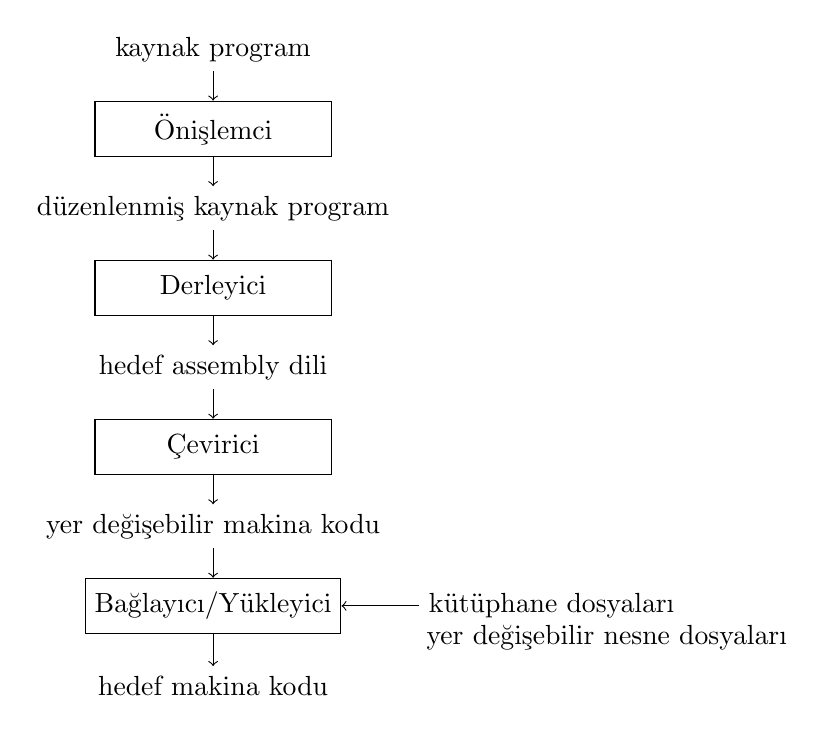
\begin{tikzpicture}[->]

\tikzstyle{rect} = [rectangle, minimum width=3cm, minimum height=0.7cm,text centered, draw=black]

\node (src_p)   {kaynak program};
\node (prep) [rect, below of=src_p, yshift=-0.01cm] {Önişlemci};   
\node (msrc_p) [below of=prep, yshift=-0.01cm]{düzenlenmiş kaynak program};
\node (cp) [rect, below of=msrc_p, yshift=-0.01cm] {Derleyici};   
\node (tr_a) [below of=cp, yshift=-0.01cm] {hedef assembly dili};
\node (as) [rect, below of=tr_a, yshift=-0.01cm]{Çevirici};   
\node (rl)  [below of=as, yshift=-0.01cm]{yer değişebilir makina kodu};
\node (ln) [rect, below of=rl, yshift=-0.01cm] {Bağlayıcı/Yükleyici};  
\node (lib) [left of=ln, xshift=6cm, yshift = -0.4cm] {yer değişebilir nesne dosyaları};
\node (lib) [left of=ln, xshift=5.3cm] {kütüphane dosyaları};
\node (out) [below of=ln, yshift=-0.01cm] {hedef makina kodu};

\draw [black](src_p) -- (prep);  
\draw [black](prep) -- (msrc_p);  
\draw [black](msrc_p) -- (cp);  
\draw [black](cp) -- (tr_a);  
\draw [black](tr_a) -- (as);  
\draw [black](as) -- (rl); 
\draw [black](rl) -- (ln);
\draw [black](ln) -- (out);
\draw [black](lib) -- (ln);   

\end{tikzpicture}

Şekil 1.5: Bir dil-işleme sistemi
\end{center}